\documentclass[12pt]{ltjsarticle}

% 基本パッケージ
\usepackage[utf8]{inputenc}
\usepackage{luatexja}
\usepackage{amsmath, amssymb}
\usepackage{graphicx}
\usepackage{geometry}

% 表のデザインを向上させるパッケージ
\usepackage{tikz}
\usetikzlibrary{arrows.meta, positioning}
\usepackage{booktabs}
\usepackage{tabularx}
\usepackage{longtable}
\usepackage{array}
\usepackage{makecell}

% セクションやタイトルのデザイン調整
\usepackage{titlesec}
\titleformat{\section}{\normalfont\Large\bfseries}{\thesection}{1em}{}
\titleformat{\subsection}{\normalfont\large\bfseries}{\thesubsection}{1em}{}
\titleformat{\subsubsection}{\normalfont\normalsize\bfseries}{\thesubsubsection}{1em}{}

\usepackage{enumitem}
\usepackage{fontspec}

\usepackage[
  colorlinks=true,
  linkcolor=blue,
  urlcolor=cyan,
  citecolor=green
]{hyperref}

\usepackage{listing}
\usepackage{xcolor}
\newcommand{\code}[1]{\colorbox{gray!20}{\texttt{#1}}}
\usepackage{float}
\geometry{top=2cm, bottom=2cm, left=2cm, right=2cm}
\usepackage{minted}

\usemintedstyle{vs}
\setminted{
    linenos,
    frame=single,
    framesep=2mm,
    baselinestretch=1.2,
    fontsize=\small,
    breaklines
}

% 数式
\usepackage{bm}

% 画像
\usepackage{float}

\begin{document}

\title{SportEase(スポーティーズ) 管理者操作説明書}
\author{行事委員会 佐藤佑作 s2301059}
\date{\today}
\maketitle
\tableofcontents

\newpage

% =====================================================================
\section{はじめに}
% =====================================================================

本書は、SportEase（スポーティーズ）の\textbf{root権限を持つ管理者}向けの操作説明書である。
rootアカウントは最上位の権限であり、大会の全体設定・システム管理・ユーザー管理など、
通常のadminやstudentでは操作できない機能にアクセスできる。

\subsection*{権限の種類}
\begin{itemize}
  \item \textbf{root} ── 本書が対象とする最上位権限。すべての機能にアクセス可能。
  \item \textbf{admin} ── 試合進行・結果入力など大会運営補助が可能。
  \item \textbf{student} ── マイページ・競技情報・トーナメント・通知などの参加者向け機能を利用できる基本権限。
\end{itemize}

rootダッシュボードは \code{/dashboard/root/} 以下の各ページから操作する。
rootでないアカウントでアクセスしようとした場合は、自動的に \code{/dashboard} へリダイレクトされる。

\subsection{大会設定の全体フロー}

大会を開催するまでの設定作業は、以下の順序で行う。
各手順の詳細は対応するセクションを参照すること。
\begin{center}
\begin{tikzpicture}[
  node distance=1.3cm,
  main/.style={
    rectangle, draw, rounded corners=4pt,
    minimum width=10cm, minimum height=0.9cm,
    text centered, fill=blue!8, font=\bfseries
  },
  arr/.style={->, thick, >=Stealth}
]
\node[main] (s1) {① 大会設定（大会作成）　→ 第\ref{sec:event}章};
\node[main, below of=s1] (s2) {② クラス人数設定　→ 第\ref{sec:classcount}章};
\node[main, below of=s2] (s3) {③ 競技登録・大会競技割り当て（定員・MD詳細含む）　→ 第\ref{sec:sport}章};
\node[main, below of=s3] (s4) {④ 競技要項PDFアップロード　→ 第\ref{sec:guidelines}章};
\node[main, below of=s4] (s5) {⑤ トーナメント生成　→ 第\ref{sec:tournament}章};
\node[main, below of=s5] (s6) {⑥ 昼競技設定　→ 第\ref{sec:noon}章};

\draw[arr] (s1) -- (s2);
\draw[arr] (s2) -- (s3);
\draw[arr] (s3) -- (s4);
\draw[arr] (s4) -- (s5);
\draw[arr] (s5) -- (s6);

\end{tikzpicture}
\end{center}

\subsection{初回ログイン}

\href{https://nitsche-gyouji.com}{https://nitsche-gyouji.com} をお好みのブラウザで開いてください。
すると、以下のような画面にアクセスできます。

\begin{figure}[H]
  \centering
  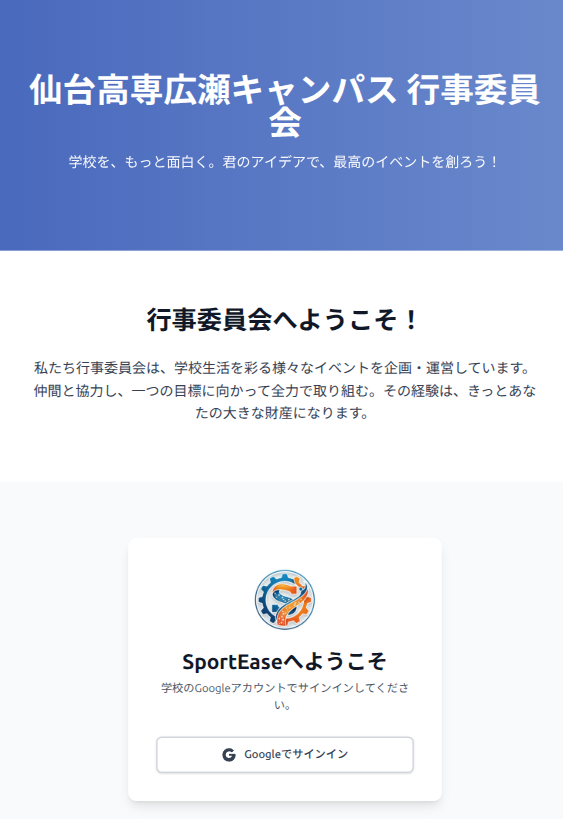
\includegraphics[width=0.8\textwidth]{./images/HP_first.png}
  \caption{アクセス結果}
\end{figure}

\texttt{Googleでサインイン}をクリックしてください。\\
\textcolor{red}{※学校のGoogle アカウントを必ず選択してください。学校のアカウント以外を選択してしまった場合は、ブラウザのキャッシュをクリアして再度アクセスしてください。}

サインインが成功すると、以下のように表示名とクラスを設定する画面に移ります。

\begin{figure}[H]
  \centering
  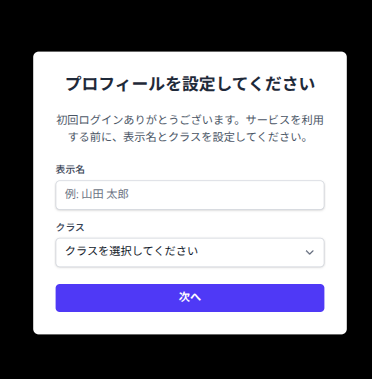
\includegraphics[width=0.8\textwidth]{./images/set-display-name.png}
  \caption{表示名とクラス設定画面}
\end{figure}

ここで、アプリないでの表示名とクラスを決定してください。
確認画面も表示されるので、クラスに関しては間違えないようにお願いします。



\newpage

% =====================================================================
\section{大会情報管理}\label{sec:event}
% =====================================================================

\textbf{ページ}: \code{/dashboard/root/event-management}

大会（イベント）の作成・設定・状態管理を行う中心的な機能である。

\subsection{大会の作成}

新規大会を作成する際は以下の項目を設定する。

\begin{itemize}
  \item \textbf{年度} ── 対象となる学年度（例：2025）
  \item \textbf{シーズン} ── 春季・秋季などの区分
  \item \textbf{開催期間} ── 大会の開始日・終了日
  \item \textbf{アンケートURL} ── 大会終了後に学生へ案内するアンケートのURL
\end{itemize}

\begin{figure}[H]
  \centering
  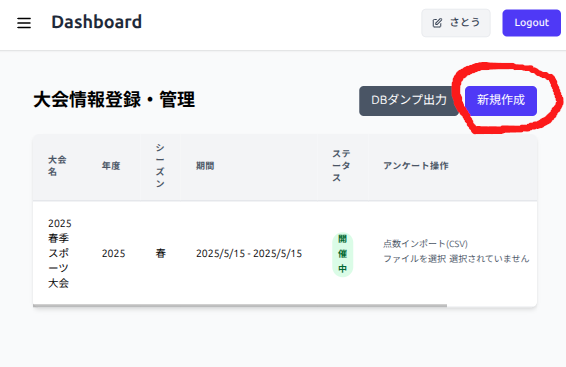
\includegraphics[width=0.8\textwidth]{./images/root-event-manage-create-1.png}
  \caption{大会作成ボタン}
\end{figure}

\begin{figure}[H]
  \centering
  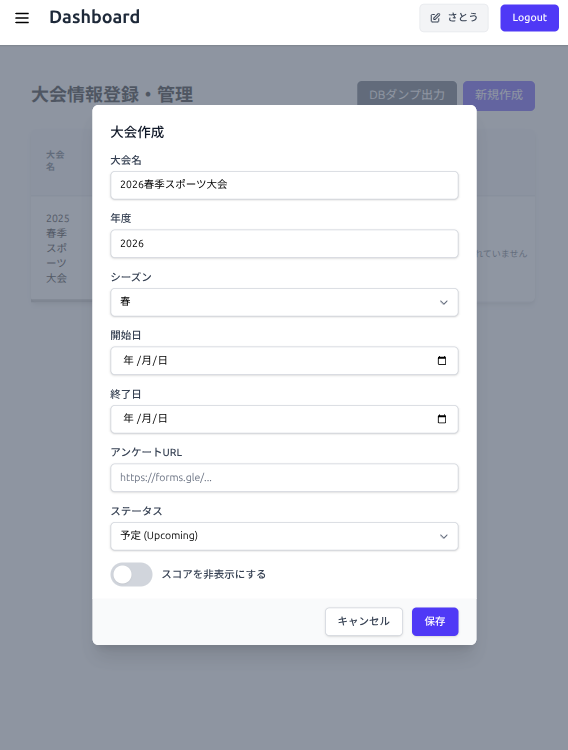
\includegraphics[width=0.8\textwidth]{./images/root-event-manage-create-2.png}
  \caption{大会概要設定画面}
\end{figure}

\subsection{大会ステータスの管理}

大会には以下の3つのステータスがあり、rootのみが変更できる。

\begin{center}
\begin{tabular}{lp{10cm}}
\toprule
\textbf{ステータス} & \textbf{説明} \\
\midrule
\code{upcoming} & 開催前。エントリー受付中の状態。 \\
\code{active}   & 開催中。試合進行・スコア入力が可能な状態。同時にactiveにできる大会は1つのみ。 \\
\code{archived} & 終了済み。結果は参照のみ可能。 \\
\bottomrule
\end{tabular}
\end{center}

\subsection{スコア非表示設定}

大会名をクリックすると、大会作成時と同じ画面が出現し、大会設定を変更することが出来る。 \\
大会ごとに、学生に対してスコア（得点）情報を非表示にするオプションを設定できる。
非表示にした場合、studentはスコアを閲覧できなくなる。

\begin{figure}[H]
  \centering
  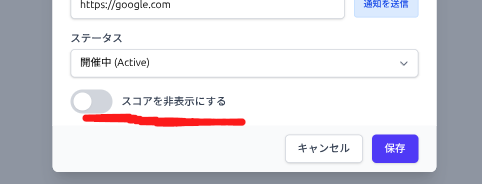
\includegraphics[width=0.8\textwidth]{./images/root-change-score-visibility-1.png}
  \caption{スコア非表示設定}
\end{figure}

\subsection{アンケート通知の配信}

大会に設定したアンケートURLを、システム全体の通知として一斉配信できる。(閉会式で一斉配信することを推奨する) \\
配信後、学生のダッシュボードに通知として表示される。

\begin{figure}[H]
  \centering
  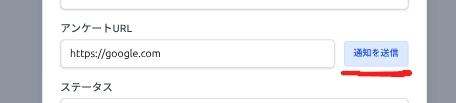
\includegraphics[width=0.8\textwidth]{./images/root-survey-distribution.png}
  \caption{アンケート通知URL設定と配信}
\end{figure}

\subsection{アンケート得点のためのCSVインポート（春季限定）}

春季大会においては、外部で集計した得点データをCSV形式でインポートできる。
CSVのフォーマットは以下の形式に従う。\\

\noindent\texttt{タイムスタンプ,クラス名,氏名} \\
\texttt{2025/01/01, IS2, 愛子太郎} \\

アンケート得点の点数変換ロジック
\begin{table}[H]
  \centering
  \begin{tabular}{|c|c|}
    得点率 & 点数 \\
    90\%以上 & 10点 \\
    80\%以上 & 9点 \\
    70\%以上 & 8点 \\
    60\%以上 & 7点 \\
    50\%以上 & 6点 \\
    50\%未満 & 5点
  \end{tabular}
  \caption{アンケート得点のための変換ロジック}
\end{table}


\subsection{結果出力（CSV・PDF）}

大会のクラス別スコア集計をCSVまたはPDF形式でダウンロードできる。
最終結果の記録・報告に利用する。

\begin{figure}[H]
  \centering
  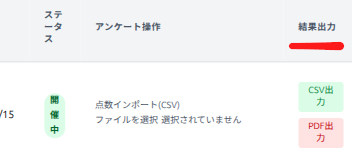
\includegraphics[width=0.8\textwidth]{./images/root-export-result.png}
  \caption{結果出力}
\end{figure}

\subsection{データベースダンプの出力}

システム全体のデータベースをSQL形式でエクスポートする機能が提供されている。
バックアップや引き継ぎ時のデータ移行に使用する。
この操作はroot専用であり、慎重に取り扱うこと。

\begin{figure}[H]
  \centering
  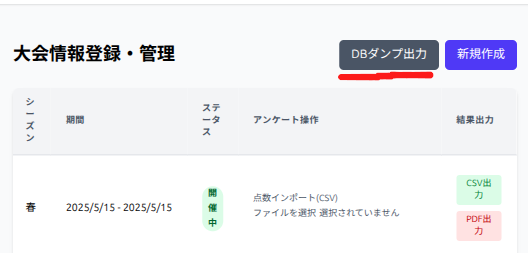
\includegraphics[width=0.8\textwidth]{./images/root-db-dump.png}
  \caption{データベースダンプ}
\end{figure}

\newpage

% =====================================================================
\section{クラス人数設定}\label{sec:classcount}
% =====================================================================

\textbf{ページ}: \code{/dashboard/root/class-student-count}

各クラスの登録学生数を設定する。
この数値は定員判定やアンケート点に使用される。

\begin{figure}[H]
  \centering
  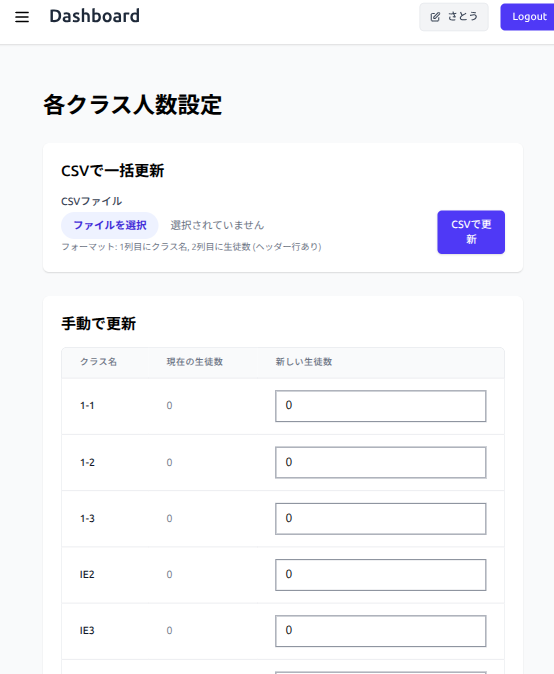
\includegraphics[width=0.8\textwidth]{./images/root-set-class-people.png}
  \caption{クラス人数設定}
\end{figure}

\subsection{個別入力による更新}

クラスを選択して学生数を手動で入力し、更新する。

\subsection{CSVによる一括更新}

\code{クラス名,学生数} 形式のCSVをアップロードすることで、
全クラスの人数を一度に更新できる。

\begin{table}[H]
  \centering
  \begin{tabular}{|c|c|}
    クラス名 & 生徒数 \\
    1-1 & 40 \\
    1-2 & 45 \\
    ... & ...
  \end{tabular}
  \caption{各クラス人数設定のCSVフォーマット例}
\end{table}

\newpage

% =====================================================================
\section{競技マスタ・大会競技管理}\label{sec:sport}
% =====================================================================

\textbf{ページ}: \code{/dashboard/root/sport-management}

競技（スポーツ種目）のマスタデータ管理と、大会への競技割り当てを行う。

\begin{figure}[H]
  \centering
  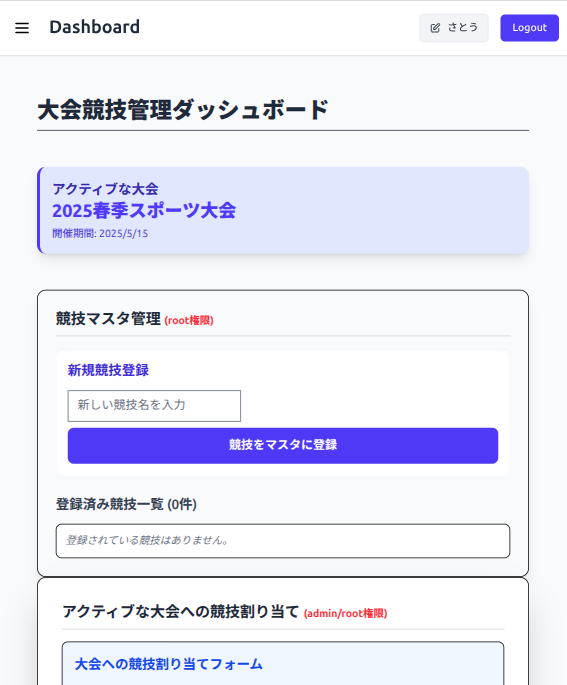
\includegraphics[width=0.8\textwidth]{./images/root-setting-competition.png}
  \caption{競技マスタ・大会競技管理画面}
\end{figure}

\subsection{競技マスタへの登録（root限定）}

システム全体で使用する競技の種目名を新規登録する。
一度登録した競技はマスタとして保持され、複数の大会で再利用できる。

\subsection{大会への競技割り当て（root・admin共通）}

アクティブな大会に対して、マスタに登録された競技を割り当てる。
割り当て時に以下の項目を設定する。

\begin{itemize}
  \item \textbf{開催場所} ── (第一体育館)gym1 / (第二体育館)gym2 / (グラウンド)ground / (その他)other から選択
  \item \textbf{競技概要・ルール} ── Markdown形式で詳細を記述(pdfアップロードも可能)
  \item \textbf{最低定員・最高定員} ── 1チームあたりの参加人数の範囲(後のQRコード機能にリンクする)
\end{itemize}

割り当て済みの競技は解除することもできる。

\newpage

% =====================================================================
\section{大会要項のアップロード}\label{sec:guidelines}
% =====================================================================

\textbf{ページ}: \code{/dashboard/root/competition-guidelines-upload}

大会の大会要項をPDFファイルとしてアップロードし、学生が参照できる状態にする。

\begin{figure}[H]
  \centering
  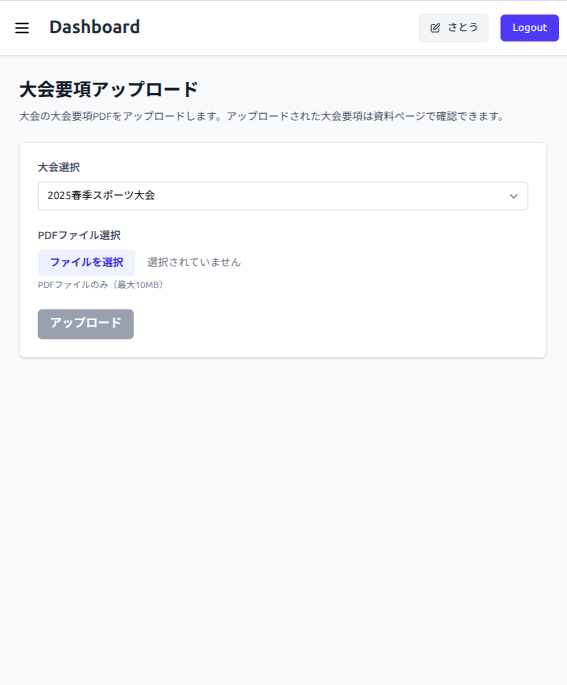
\includegraphics[width=0.8\textwidth]{./images/root-event-guideline-upload.png}
  \caption{大会要項アップロード画面}
\end{figure}

\subsection{PDFのアップロード・更新}

アクティブな大会に対して競技要項PDFをアップロードする。
既存のPDFは上書き（置換）することができる。

\subsection{PDFの削除}

登録済みのPDFを削除することもできる。

\begin{figure}[H]
  \centering
  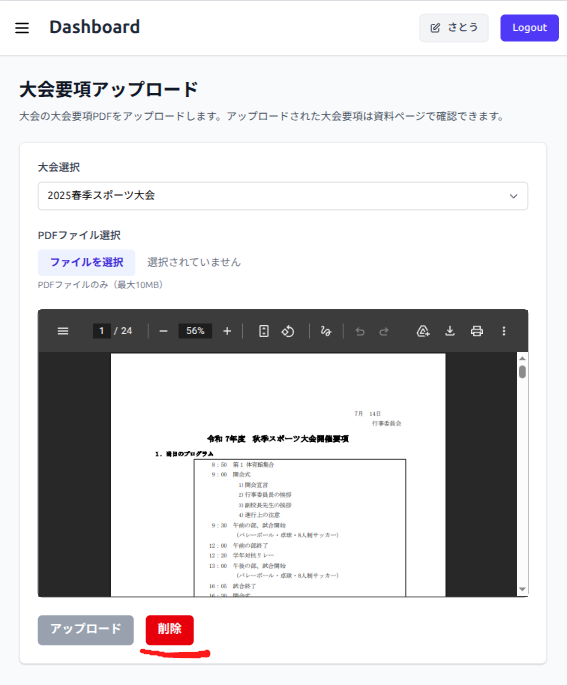
\includegraphics[width=0.8\textwidth]{./images/root-setting-competition-remove.png}
  \caption{大会要項PDFの削除}
\end{figure}

\subsection{学生側での参照}

アップロードされたPDFは学生のダッシュボードからアクセス可能となる。
最新の要項に更新した場合は即時に反映される。

\newpage

% =====================================================================
\section{トーナメント生成・管理}\label{sec:tournament}
% =====================================================================

\textbf{ページ}: \code{/dashboard/root/tournament-management}

大会の全競技にわたるトーナメント（試合組み合わせ表）を自動生成する。

\begin{figure}[H]
  \centering
  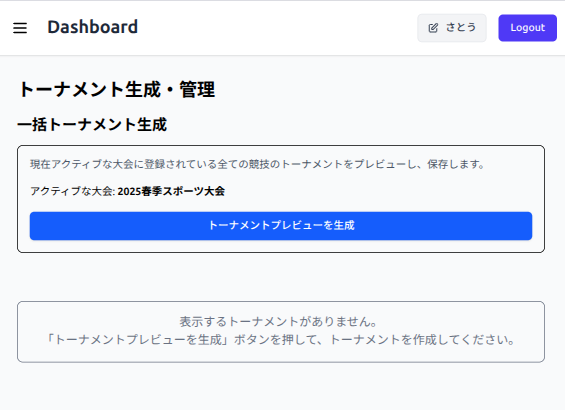
\includegraphics[width=0.8\textwidth]{./images/root-generate-tournament-screen.png}
  \caption{トーナメント生成画面}
\end{figure}

\subsection{トーナメントの自動生成}

クラスの人数・エントリー状況をもとに、全競技のトーナメントブラケットを一括生成する。
生成処理はバックエンドで行われ、シード順・クラス振り分けも自動で決定される。

\subsection{プレビューの確認}

実際にデータベースへ保存する前に、生成結果をプレビューとして確認できる。
対戦組み合わせや試合数に問題がないかを確認してから確定する。

\begin{figure}[H]
  \centering
  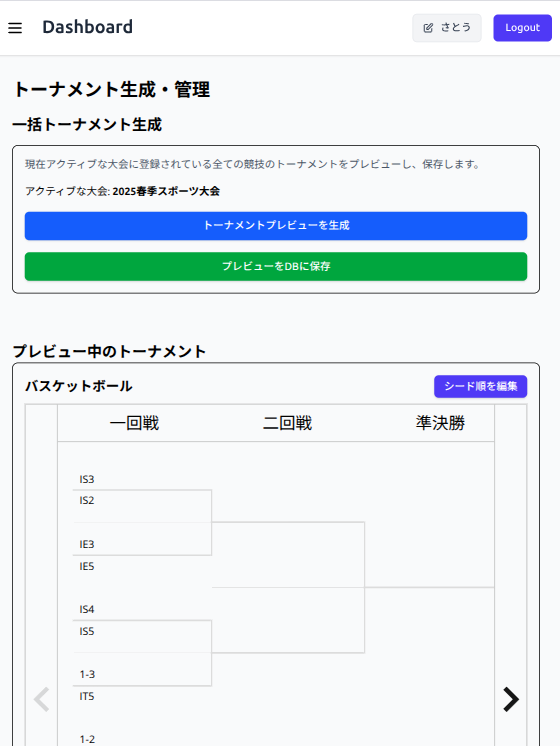
\includegraphics[width=0.8\textwidth]{./images/root-tournament-preview.png}
  \caption{トーナメントプレビュー}
\end{figure}

トーナメントを任意に編集することもできる。図14のシード順を編集をクリックすることで、以下の画面になりドラッグ\&ドロップで操作できる。

\begin{figure}[H]
  \centering
  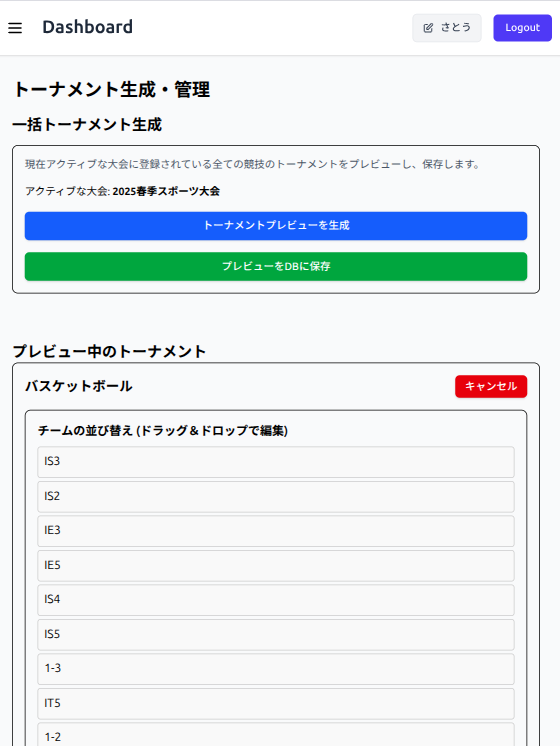
\includegraphics[width=0.8\textwidth]{./images/root-tournament-edit.png}
  \caption{トーナメント編集画面}
\end{figure}

\begin{figure}[H]
  \centering
  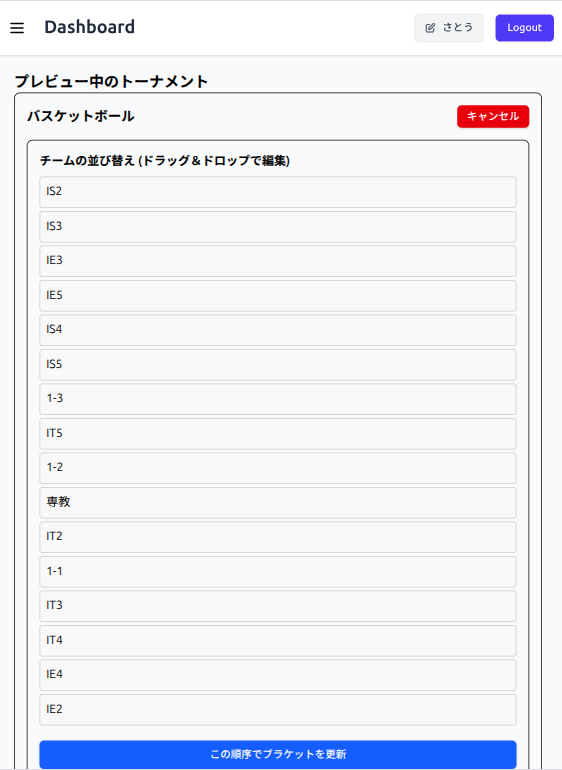
\includegraphics[width=0.8\textwidth]{./images/root-tournament-edit-update.png}
  \caption{トーナメント編集後確定}
\end{figure}

\subsection{プレビューの保存・確定}

プレビューの内容を確認後、「保存」操作でデータベースに書き込む。
保存後はトーナメントブラケットが各ページに反映される。

\newpage

% =====================================================================
\section{昼競技（Noon Game）管理}\label{sec:noon}
% =====================================================================

\textbf{ページ}: \code{/dashboard/root/noon-game}

昼休みに行われる特別競技（昼競技）の設定・進行管理を行う。いくつかのテンプレートから選択することも出来る。

\begin{figure}[H]
  \centering
  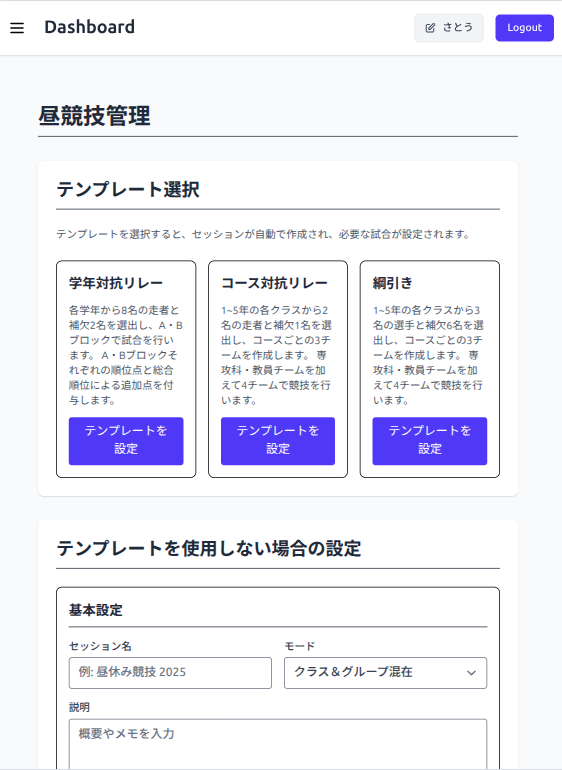
\includegraphics[width=0.8\textwidth]{./images/root-noon-screen.png}
  \caption{昼競技設定画面スクリーン}
\end{figure}

\subsection{セッション管理}

昼競技の開催枠（セッション）を作成・管理する。
セッションごとに以下を設定する。

\begin{itemize}
  \item \textbf{セッション名・説明}
  \item \textbf{ポイント設定} ── 勝利・敗北・引き分け・参加ポイントの各値
  \item \textbf{手動ポイント追加の有効化} ── 特別な加点が必要な場合に利用
\end{itemize}

\subsection{グループ管理}

参加クラスをグループに振り分ける。
グループの作成・更新・削除が可能であり、ラウンドロビン形式の対戦に使用される。

\subsection{マッチ管理}

各試合（マッチ）の以下の情報を管理する。

\begin{itemize}
  \item 試合日時・場所
  \item 試合フォーマット（時間制・得点制など）
  \item 試合ステータス（予定 / 進行中 / 終了）
\end{itemize}

\subsection{テンプレートの実行}

昼競技には定型的な種目に対応したテンプレートが用意されている。

\begin{itemize}
  \item \textbf{年リレー} ── 学年別リレーの試合設定テンプレート
  \item \textbf{コースリレー} ── コース別リレーの試合設定テンプレート
  \item \textbf{綱引き} ── 綱引きの試合設定テンプレート
\end{itemize}

テンプレートを実行すると、対戦カードが自動的に生成される。
結果はテンプレートランに記録する。

\subsection{手動ポイント追加}

セッションに手動加点機能が有効な場合、特定のクラスに対して任意のポイントを追加できる。

\newpage

% =====================================================================
\section{雨天時モード管理}
% =====================================================================

\textbf{ページ}: \code{/dashboard/root/rainy-mode}

雨天時に競技プログラムを変更するための専用設定である。

\begin{figure}[H]
  \centering
  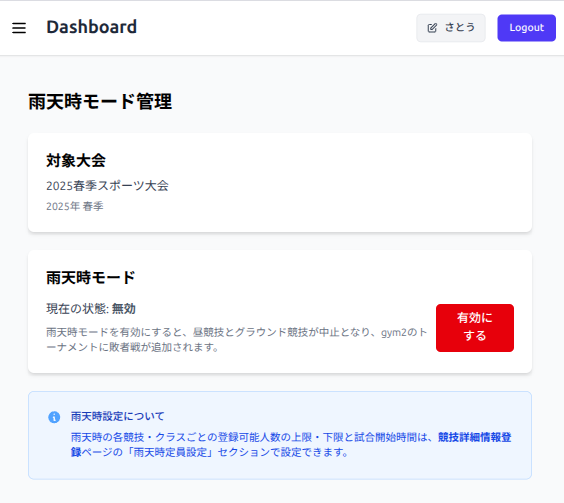
\includegraphics[width=0.8\textwidth]{./images/root-rain-mode.png}
  \caption{雨天時モード画面}
\end{figure}

\subsection{雨天時モードのON/OFF}

雨天時モードをONにすると、以下の変更が自動的に適用される。

\begin{itemize}
  \item \textbf{昼競技（Noon Game）が中止}になる
  \item \textbf{グラウンドで行われる競技が中止}になる
  \item \textbf{Gym2のトーナメントに敗者復活戦が追加}される
\end{itemize}

モードはON/OFFのトグルで切り替えるのみであり、即時に反映される。

\subsection{雨天時定員設定}

各競技・クラスごとに、雨天時の定員（上限・下限）と試合開始時間を個別に設定できる。
設定は競技詳細登録ページから行い、雨天時モードON時のみ参照される。

\newpage

% =====================================================================
\section{通知管理}
% =====================================================================

\textbf{ページ}: \code{/dashboard/root/notification}

システム全体に対してプッシュ通知を作成・配信する機能である。

\begin{figure}[H]
  \centering
  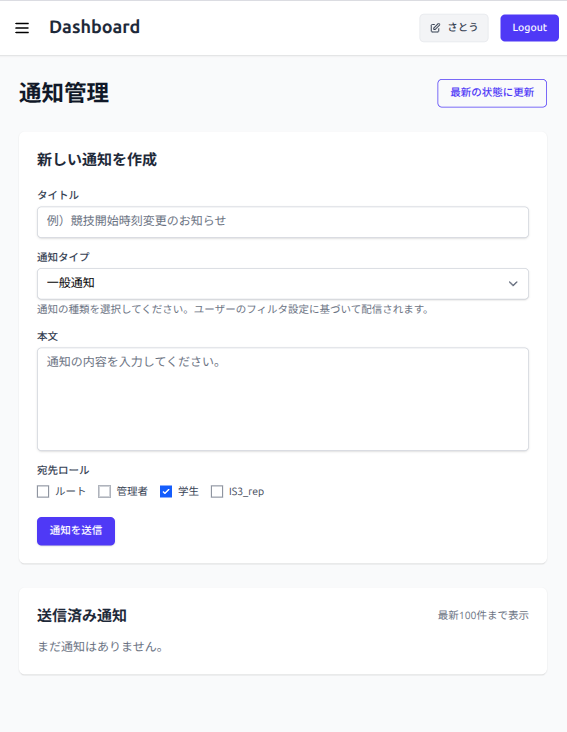
\includegraphics[width=0.8\textwidth]{./images/root-nortification-manage.png}
  \caption{通知管理画面}
\end{figure}

\subsection{通知の作成と配信}

以下の設定を行って通知を作成・送信する。

\begin{itemize}
  \item \textbf{通知タイトル・本文} ── 任意のテキストを入力
  \item \textbf{通知タイプ} ── 一般通知 / 自分のクラスの試合 / 決勝戦 / 全試合 から選択
  \item \textbf{配信先ロール} ── student・admin・root の任意の組み合わせを指定
\end{itemize}

\subsection{送信済み通知の確認}

過去に配信した通知の一覧を確認できる。
通知内容・送信日時・配信先ロールが記録されている。

\newpage

% =====================================================================
\section{通知申請管理}
% =====================================================================

\textbf{ページ}: \code{/dashboard/root/notification-requests}

学生（student）から提出された通知作成申請を審査・処理する機能である。

\begin{figure}[H]
  \centering
  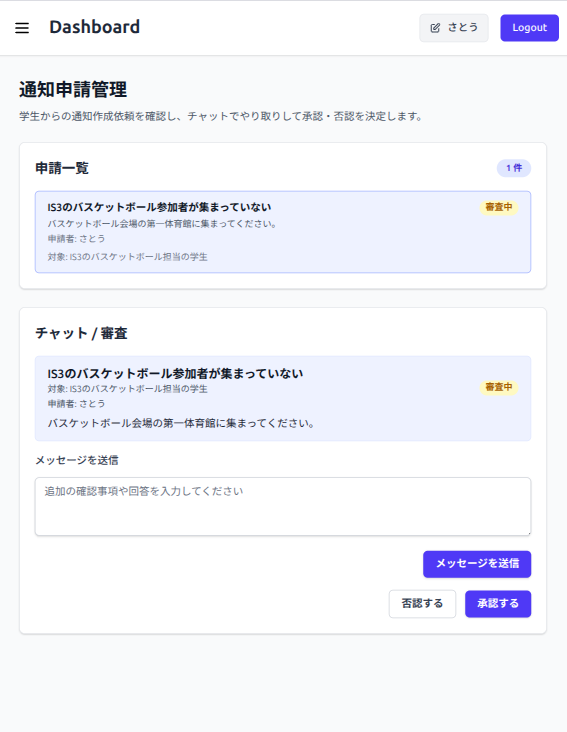
\includegraphics[width=0.8\textwidth]{./images/root-nortification-requests-manage.png}
  \caption{通知申請管理画面}
\end{figure}

\subsection{申請の確認とメッセージ交換}

申請はチャット形式のUIで表示される。
申請者とのメッセージのやり取りが可能であり、内容の確認や追加質問を行える。

\subsection{申請の承認・否認}

審査結果として「承認（approved）」または「否認（rejected）」を決定する。
承認された申請に基づき、rootが通知を配信する。

\newpage

% =====================================================================
\section{ユーザー管理}
% =====================================================================

\textbf{ページ}: \code{/dashboard/root/change-username}

システム利用者の表示名やクラス所属ロールを管理する。

\begin{figure}[H]
  \centering
  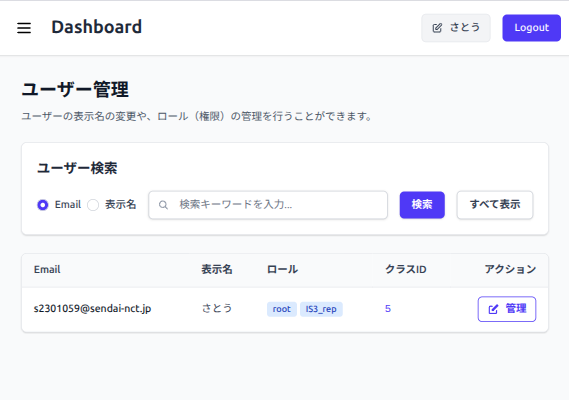
\includegraphics[width=0.8\textwidth]{./images/root-user-manage.png}
  \caption{ウーザー管理画面}
\end{figure}

\subsection{ユーザーの検索}

メールアドレスまたは表示名でユーザーを検索できる。

\subsection{表示名の変更}

対象ユーザーのシステム上の表示名を変更する。

\subsection{クラス所属ロールの付け替え}

\code{クラス名\_rep} 形式のクラス所属ロールを変更する際、
旧ロールの削除と新ロールの付与が自動的に行われる。
これにより、一人のユーザーが複数クラスに所属する状況を防ぐ。

\newpage

% =====================================================================
\section{権限管理}
% =====================================================================

\textbf{ページ}: \code{/dashboard/root/user-promotion}

ユーザーに対して \code{admin} / \code{root} の基本権限を付与・剥奪する機能である。

\subsection{ユーザーの検索}

メールアドレスまたは表示名で対象ユーザーを検索できる。

\subsection{基本権限の付与}

検索結果の一覧から、対象ユーザーに \code{admin} または \code{root} を付与できる。

\subsection{基本権限の剥奪}

既に付与されている \code{admin} または \code{root} を剥奪できる。
任意ロールの付与・削除はadminの「ロール管理」画面で行う。

\newpage

% =====================================================================
\section{MIC確認}
% =====================================================================

\textbf{ページ}: \code{/dashboard/root/identify-mic}

MIC（Most Impressive Class：最も印象を残したクラス）の確認ページである。
MICは投票によって決定され、rootはその結果を確認できる。

表示される情報は以下のとおりである。

\begin{itemize}
  \item クラス名
  \item 合計ポイント
  \item 対象シーズン情報
\end{itemize}

なお、投票自体はadminも行うことができる。

\newpage

% =====================================================================
\section{機能一覧まとめ}
% =====================================================================

以下にroot権限でのみ実行可能な操作を一覧にまとめる。

\begin{longtable}{p{4.5cm}p{9cm}}
\toprule
\textbf{機能} & \textbf{概要} \\
\midrule
\endhead
大会の作成・編集 & 年度・シーズン・期間・アンケートURLを設定して大会を登録・変更する \\
\midrule
大会ステータス変更 & upcoming / active / archived の切り替え \\
\midrule
スコア非表示設定 & 学生へのスコア公開・非公開を大会ごとに設定 \\
\midrule
アンケート通知配信 & 大会に設定したアンケートURLを全体通知として送信 \\
\midrule
得点CSVインポート & 外部集計した得点データをCSVで取り込む（春季限定） \\
\midrule
結果のCSV/PDF出力 & クラス別スコア集計を外部ファイルとして出力 \\
\midrule
DBダンプ出力 & データベース全体をSQL形式でエクスポート \\
\midrule
雨天時モード切替 & 昼競技・グラウンド競技の中止、敗者復活戦追加を一括制御 \\
\midrule
雨天時定員設定 & 競技・クラスごとの雨天時定員・開始時間を個別設定 \\
\midrule
競技マスタ登録 & 全大会で利用できる競技種目をシステムに登録 \\
\midrule
大会への競技割り当て & 場所・ルール・定員を設定して競技を大会に紐付け \\
\midrule
通知作成・配信 & タイプ・配信先ロールを指定してプッシュ通知を送信 \\
\midrule
通知申請の承認・否認 & 学生からの通知申請をチャット形式で審査し決定 \\
\midrule
トーナメント自動生成 & 全競技のトーナメントブラケットをプレビュー確認後に確定 \\
\midrule
昼競技セッション管理 & 昼競技の開催枠・ポイント設定・グループ・マッチを管理 \\
\midrule
昼競技テンプレート実行 & 年リレー・コースリレー・綱引きの対戦カードを自動生成 \\
\midrule
ユーザー表示名変更 & 任意ユーザーのシステム表示名を更新 \\
\midrule
ユーザーロール付与・削除 & student / admin / root ロールの追加・削除 \\
\midrule
クラス所属ロール付け替え & クラス所属ロールの変更（旧ロール自動削除） \\
\midrule
クラス人数設定 & 各クラスの登録学生数を手動またはCSVで更新 \\
\midrule
MIC結果確認 & 投票により決定されたMICクラスの情報を確認 \\
\midrule
競技要項PDFアップロード & 大会の競技要項PDFを登録・更新・削除 \\
\bottomrule
\end{longtable}

\end{document}
